\subsection{QuizziPedia::Back-End}
\subsubsection{Informazioni generali}
\label{QuizziPedia::Back-End}
\begin{figure}[ht]
	\centering
	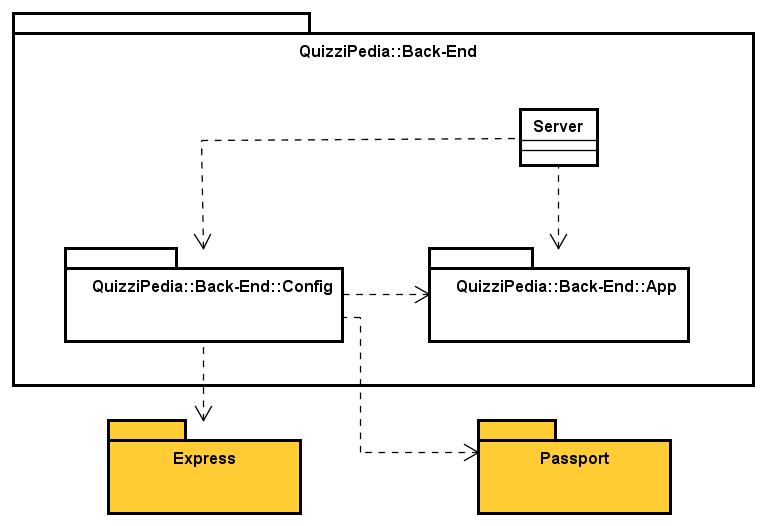
\includegraphics[scale=0.7]{UML/Package/QuizziPedia_Back-End.png}
	\caption{QuizziPedia::Back-End}
\end{figure}
\FloatBarrier
	\begin{itemize}
		\item \textbf{Descrizione}:
		\textit{package\ped{G}} contenenti le componenti della parte back-end dell'applicazione;
		\item \textbf{Package contenuti}:
		\begin{itemize}
			\item \texttt{App}:
			\textit{package\ped{G}} contenente le componenti del \textit{server\ped{G}} che implementano il \textit{pattern MVC\ped{G}};
			\item \texttt{Config}:
			\textit{package\ped{G}} contenente le componenti di configurazione del \textit{server\ped{G}}.
		\end{itemize}
	\end{itemize}
\subsubsection{Classi}
	\paragraph{QuizziPedia::Back-End::Server}
\label{QuizziPedia::Back-End::Server}
\begin{figure}[ht]
	\centering
	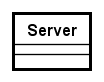
\includegraphics[scale=0.8]{UML/Classi/Back-End/QuizziPedia_Back-End_Server.png}
	\caption{QuizziPedia::Back-End::Server}
\end{figure}
\FloatBarrier
	\begin{itemize}
		\item \textbf{Descrizione}:
		classe che avvia il \textit{server\ped{G}}. Nello specifico apre una connessione al database tramite \textit{Mongoose\ped{G}}, invoca il \textit{middleware\ped{G}} \textit{Express\ped{G}} passando un riferimento al database \textit{MongoDB\ped{G}} come parametro in modo  che possa configurarsi con esso, invoca il \textit{middleware\ped{G}} \textit{Passport\ped{G}} ed infine si mette in ascolto su una determinata porta. E' il componente \textit{client\ped{G}} del \textit{design pattern\ped{G}} \textit{Chain of responsibility\ped{G}}. Utilizza i moduli \textit{Mongoose\ped{G}}, \textit{Express\ped{G}}, \textit{Passport\ped{G}};
		\item \textbf{Utilizzo}:
		utilizzo per avviare l'applicazione lato \textit{server\ped{G}}. Inizializza, internamente al back-end, la catena di gestione delle chiamate \textit{REST\ped{G}} utilizzando le classi contenute nel \textit{package\ped{G}} \texttt{Routers}.
	\end{itemize}
	